\section{Section Title}
\label{sec:N_SECTION_1}

Introductory paragraph for this section. Reference other chapters with \cref{ch:N} and cite
sources with~\cite{key}. Use \gls{acronym} for the first occurrence of a defined acronym and
\gls{term} for glossary terms.

\subsection{Equations}
\label{sec:N_SECTION_1_EQUATIONS}

Inline math: $E = mc^2$. Display equations with automatic numbering:

\begin{align}
  \label{eq:N_example}
  f(x) &= \int_0^\infty g(x, t) \, dt \\
       &= A \cdot e^{-\lambda x}
\end{align}

Reference as \cref{eq:N_example}. Use \texttt{siunitx} for quantities with units:
$m = \SI{1.5}{\kilo\gram}$, $E = \SI{7}{\tera\electronvolt}$.

\subsection{Figures}
\label{sec:N_SECTION_1_FIGURES}

\begin{figure}[!ht]
  \centering
  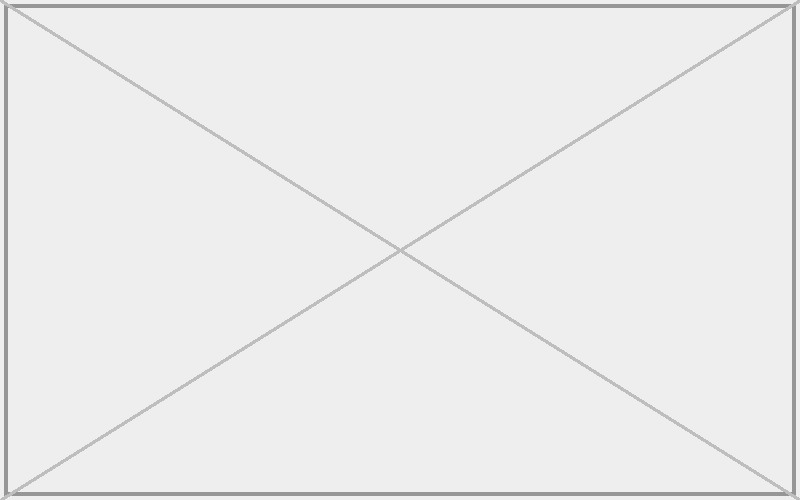
\includegraphics[width=0.7\textwidth]{figures/placeholder.png}
  \caption{Figure caption. Describe what is shown and highlight the key takeaway.}
  \label{fig:N_example}
\end{figure}

Reference as \cref{fig:N_example}. For side-by-side panels use the \texttt{subcaption}
package:

\begin{figure}[!ht]
  \centering
  \begin{subfigure}[b]{0.48\textwidth}
    \centering
    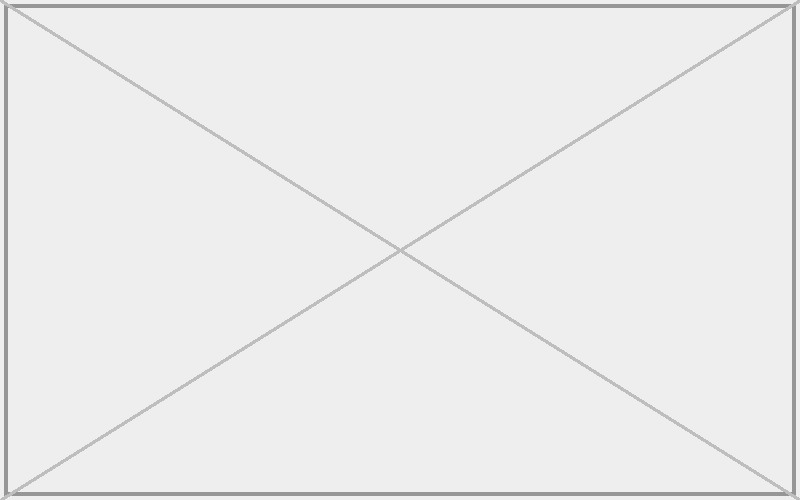
\includegraphics[width=0.9\textwidth]{figures/placeholder.png}
    \caption{Left panel.}
    \label{fig:N_example_left}
  \end{subfigure}
  \hfill
  \begin{subfigure}[b]{0.48\textwidth}
    \centering
    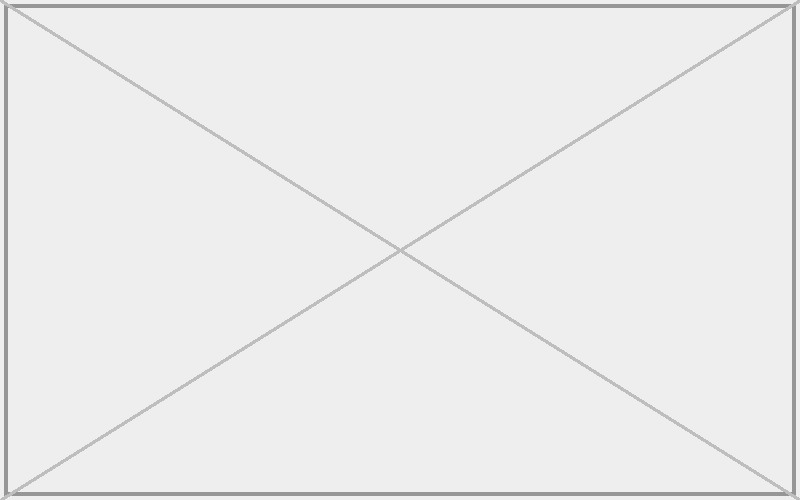
\includegraphics[width=0.9\textwidth]{figures/placeholder.png}
    \caption{Right panel.}
    \label{fig:N_example_right}
  \end{subfigure}
  \caption{Combined figure caption.}
  \label{fig:N_example_combined}
\end{figure}
